The composability of localization protocols proposed in~\cite{composability} tries to leverage the weaknesses that some protocols may have under certain conditions. Nevertheless, there might be opportunities where the predefined sequence of protocol execution would result in increased errors due to lack of consideration of the \emph{unknown} node's network-environment or the priorities of the deployment.

We propose a localization procedure which focuses on considering the protocols' best-working environmental conditions and the WSN deployment considerations in order to make the most beneficial protocol selection instead of a static sequential execution.

\begin{figure*}[tb]
  \centering
  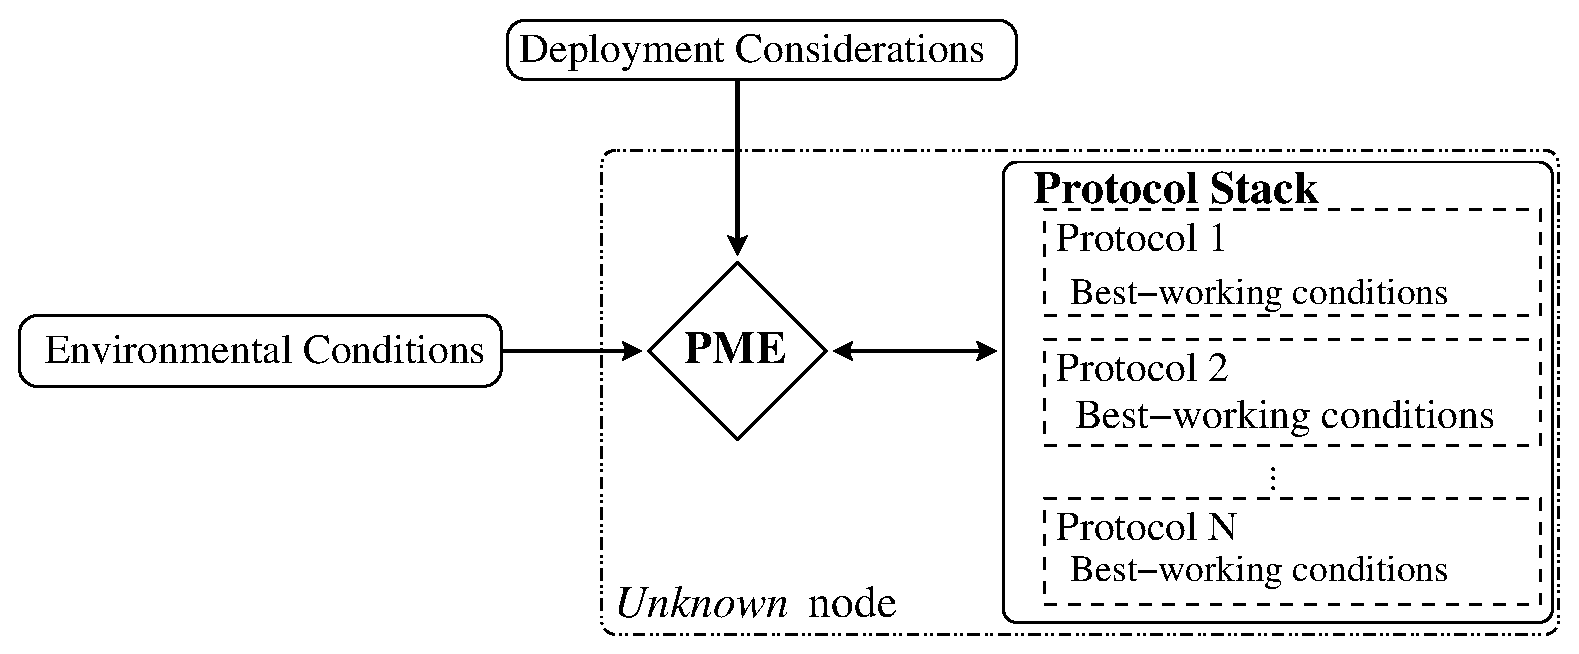
\includegraphics[width=0.83\linewidth]{section3/figures/LocProc_small.eps}
  \caption{Localization procedure: architecture
  \label{fig:LocProc}}
\end{figure*}

\subsection{Best-working environmental conditions}\label{bestWorkingConditions}
Some protocols perform better than others under different conditions. For instance, some \emph{Anchor}-based localization techniques (like the ones described in Section~\ref{literature}) require more connections to \emph{Anchors} than others~\cite{rang:loc:techniques}.

When referring to best-working environmental conditions, it is to point out network-environment metrics that would help a determined localization protocol to work more efficiently, like: number of effective connections of the type \emph{unknown-Anchor}, current delay, available bandwidth, network size or processing capabilities of the nodes.

Up-to-date information of the node's environmental conditions aids the process of determining which localization protocol is more capable of achieving the deployment considerations.

\subsection{Deployment considerations}\label{deploymentConsiderations}
Each deployment has defined goals and restrictions, like: long/coarse network lifetime, high/coarse accuracy, short/coarse localization traffic overhead or high/low localization protocol convergence time. These are tightly related to the application running over it.

Each localization protocol has its best-working environmental conditions, that when complied allow the protocol to provide satisfactory results and follow the deployment considerations.

\subsection{Pattern Matching Engine (PME)}\label{PME}
Is a module inside the localization procedure responsible for translating the \emph{unknown} node's environmental conditions into localization protocols than could comply with the deployment considerations. That is, for certain deployment considerations the PME will select a set of appropriate localization protocols where their best-working environmental conditions are met. If all the conditions are satisfied, the PME prioritizes the protocol that better complies with the deployment considerations. 

The architecture of the localization procedure is shown in Fig.~\ref{fig:LocProc}, whence it can be appreciated the PME gathering environmental conditions and deployment considerations to select the appropriate localization protocols.

%shows an overview of the localization procedure's architecture and highlights the role of the PME.